%%%%%%%%%%%%%%%%%%%%%%%%%%%%%%%%%%%%%%%%%%%%%%%%%%%%
%%%             Metadata                         %%%
%%%%%%%%%%%%%%%%%%%%%%%%%%%%%%%%%%%%%%%%%%%%%%%%%%%%      

\title{Grundkurs Linguistik}

\subtitle{Phonetik\\
Sprechaktlautlehre}

\author[aMyP]{
	{\small Antonio Machicao y Priemer}
%	\\
%	{\footnotesize \url{http://www.linguistik.hu-berlin.de/staff/amyp}\\
%	\href{mailto:mapriema@hu-berlin.de}{mapriema@hu-berlin.de}}
}

\institute{Institut für deutsche Sprache und Linguistik}

%%%%%%%%%%%%%%%%%%%%%%%%%      
\date{ }
%\publishers{\textbf{6. linguistischer Methodenworkshop \\ Humboldt-Universität zu Berlin}}

%\hyphenation{nobreak}


%%%%%%%%%%%%%%%%%%%%%%%%%%%%%%%%%%%%%%%%%%%%%%%%%%%%
%%%             Preamble's End                   %%%
%%%%%%%%%%%%%%%%%%%%%%%%%%%%%%%%%%%%%%%%%%%%%%%%%%%%      


%%%%%%%%%%%%%%%%%%%%%%%%%      
\huberlintitlepage

\iftoggle{toc}{
\frame{
\begin{multicols}{2}
	\frametitle{Inhaltsverzeichnis}\tableofcontents
	%[pausesections]
\end{multicols}
}
}

%%%%%%%%%%%%%%%%%%%%%%%%%%%%%%%%%%%
%%%%%%%%%%%%%%%%%%%%%%%%%%%%%%%%%%

\nocite{Hall00a} 
\nocite{Hall00a} 
\nocite{Repp&Co12a}
\nocite{Repp&Co12a}

%%%%%%%%%%%%%%%%%%%%%%%%%%%%%%%%%%%
%%%%%%%%%%%%%%%%%%%%%%%%%%%%%%%%%%
%
\section{Einführung}
%\frame{
%\begin{multicols}{2}
%\frametitle{~}
%	\tableofcontents[currentsection]
%\end{multicols}
%}
%%%%%%%%%%%%%%%%%%%%%%%%%%%%%%%%%%%%%%%%%%%%%%%%

\begin{frame}
\frametitle{Einführung}

	\begin{itemize}
		\item Phonetik $\approx$ \gqq{Lautlehre}, \gqq{Lehre der Sprachlaute}, \gqq{Sprechaktlautlehre}
		\item[]
		\item Sie beschäftigt sich mit der \textbf{materiellen Seite} des Sprechens $\rightarrow$ Sprachlaute 
		\item[]
		\item \textbf{Minimaleinheit} der Phonetik: \textbf{Phon} $\approx$ Sprachlaut $\approx$ Segment $\approx$ einfach nur \gqq{Laut}
		\item[]
		\item Sie zählt nicht im engeren Sinne zu den \textit{grammatischen Modulen} in der Sprachkompetenz, sondern zu dem \textbf{artikulatorisch-perzeptorischen Apparat}.
	\end{itemize}
	
\end{frame}



%%%%%%%%%%%%%%%%%%%%%%%%%%%%%%%%%%%%%%%%%%%%%%%%%%%%%%%%%%%%

\begin{frame}
\frametitle{Einführung}

	\begin{itemize}
		\item In den Sprachen der Welt zählt man insgesamt über 200 Vokale und über 500 Konsonanten.
		
		\begin{itemize}
			\item[]
			\item Pirahã: 10 Laute (eher Phoneme)\\
			\textbf{VIDEO:} \href{run:material/04SpokenPiraha.mp4}{Spoken Pirahã with subtitles}
			\item[]
			\item Hawaiisch: 11--13 Laute (eher Phoneme)
			\item[]
			\item {!}Xóõ: 141--159 Laute (eher Phoneme)
			\item[]
			\item Deutsch: 50 Laute (ung. 32 Phoneme)
		\end{itemize}
		
	\end{itemize}
	
\end{frame}



%%%%%%%%%%%%%%%%%%%%%%%%%%%%%%%%%%%%%%%%%%%%%%%%%%%%%%%%%%%%%%%%

\begin{frame}
\frametitle{Einführung}

\begin{itemize}
		\item \textbf{ÜB:} Wie viele Laute haben die folgenden Wörter?
		
		\begin{columns}
			\column{.30\textwidth}
				\begin{enumerate}
					\item \ab{Fische}
					\item \ab{Nixe}
					\item \ab{lang}
					\item \ab{Bearbeitung}
				\end{enumerate} 				
			\column{.35\textwidth}
				\begin{enumerate}
					\item<2> \textipa{[ f \textsci{} \textesh{} @ ]}
					\item<2> \textipa{[ n \textsci{} k s @ ]}
					\item<2> \textipa{[ l a N ]}
					\item<2> \textipa{[ b @ P a \textscr  b \t{aI} t \textupsilon N ]}
				\end{enumerate} 
			\column{.15\textwidth}
				\begin{enumerate}
					\item<2>[] 4
					\item<2>[] 5
					\item<2>[] 3
					\item<2>[] 10--11
                \end{enumerate}
		\end{columns}
		
\end{itemize}

\end{frame}



%%%%%%%%%%%%%%%%%%%%%%%%%%%%%%%%%%%%%%%%%%%%%%%%%%%%%%%%%%%%%%%%

\begin{frame}
\frametitle{Einführung}

	\begin{itemize}
	
		\item Methodik: \textbf{naturwissenschaftlich}
		\item Messung und Analyse physiologischer und physikalischer Aspekte der Sprache
		\item \textbf{Lautkontinuum} wird in einzelne Laute zerlegt
		\item[]
		\item Bereiche der Phonetik:

		\begin{itemize}
			\item Artikulatorische Phonetik
			\item[]
			\item Akustische Phonetik
			\item[]
			\item Auditive (perzeptive) Phonetik
		\end{itemize}
		
	\end{itemize}
	
\end{frame}



%%%%%%%%%%%%%%%%%%%%%%%%%%%%%%%%%%%%%%%%%%%%%%%%%%%%%%%%%%%%%%%%
%%%%%%%%%%%%%%%%%%%%%%%%%%%%%%%%%%%%%%%%%%%%%%%%%%%%%%%%%%%%%%%
%
\section{Bereiche der Phonetik}
%
\iftoggle{toc}{
\frame{
\begin{multicols}{2}
	\tableofcontents[currentsection]
\end{multicols}
}
}
%%%%%%%%%%%%%%%%%%%%%%%%%%%%%%%%%%%%%%%%%%%%%%%%%%%%%%%%%%%%%%%%

\begin{frame}{Bereiche der Phonetik}

	\begin{table}
	\centering 
	
		\begin{tabular}{p{0.23\linewidth}p{0.05\linewidth}p{0.23\linewidth}p{0.05\linewidth}p{0.23\linewidth}}
			\hline
			\textbf{Artikulatorische Phonetik} & & \textbf{Akustische}\par \textbf{Phonetik} & & \textbf{Auditive}\par \textbf{(perzeptive)}\par \textbf{Phonetik} \\
			\hline
  			Sprecher & & Schallsignal & & Hörer \\
			\hline
			Lautproduktion & $\rightarrow$ & Transmission & $\rightarrow$ & Perzeption\\
			\hline
		\end{tabular}
		
	\caption{Bereiche der Phonetik \citep{Ramers08a}} 
	\end{table}	
		
\end{frame}



%%%%%%%%%%%%%%%%%%%%%%%%%%%%%%%%%%%%%%%%%%%%%%%%%%%%%%%%%%%%%%%%

\begin{frame}
\frametitle{Bereiche der Phonetik}

	\begin{itemize}
		\item \textbf{Artikulatorische Phonetik}
		
		\begin{itemize}
			\item \textbf{Erzeugung} von Lautereignissen (von der Steuerung durch das Gehirn bis zu den konkreten artikulatorischen Bewegungen im Mund-, Rachen- und Nasenraum und im Kehlkopf)

			\ea Zungenbewegung bei der Aussprache des Lautes \textipa{[ \t{tS} ]}
			\z

		\end{itemize}
		
		\item[]
		\item \textbf{Akustische Phonetik}
		
		\begin{itemize}
			\item physikalische Eigenschaften von \textbf{Schallwellen}, die bei der Produktion und Übertragung von Sprachlauten auftreten

			\ea physikalische Eigenschaften eines Lauts im Übertragungsprozess: Frequenzbereich, Intensität, Länge, etc.
			\z
			
		\end{itemize}
		
	\end{itemize}
	
\end{frame}



%%%%%%%%%%%%%%%%%%%%%%%%%%%%%%%%%%%%%%%%%%%%%%%%%%%%%%%%%%%%%%%%

\begin{frame}
\frametitle{Bereiche der Phonetik}

	\begin{itemize}
	
		\item \textbf{Auditive (perzeptive) Phonetik}
		
		\begin{itemize}
			\item \textbf{Wahrnehmung} (Empfang und Verstehen) von Sprachlauten

			\ea Wie nimmt der Hörer den Unterschied zwischen den Vokalen in \ab{Beet} und \ab{Bett} wahr?
			\z
			
		\end{itemize}
		
		\item[]
	\end{itemize}
	
\end{frame}



%%%%%%%%%%%%%%%%%%%%%%%%%%%%%%%%%%%%%%%%%%%%%%%%%%%%%%%%%%%%%%%%
%%%%%%%%%%%%%%%%%%%%%%%%%%%%%%%%%%%%%%%%%%%%%%%%%%%%%%%%%%%%%%%%
%
\section{Methodik}
\iftoggle{toc}{
\frame{
\begin{multicols}{2}
	\tableofcontents[currentsection]
\end{multicols}
}
}
%%%%%%%%%%%%%%%%%%%%%%%%%%%%%%%%%%%%%%%%%%%%%%%%%%%%%%%%%%%%%%%%

\begin{frame}{Methodik}

	\begin{figure}
		\centering
		
		\includegraphics[scale=0.1]{material/04RousselotsApparatzurAufzeichnungderSprache}
		\caption{Rousselots Apparat zur Aufzeichnung der Sprache (Holzstich, um 1900). (https://de.wikipedia.org/wiki/Jean-Pierre$\_$Rousselot$\#$ /media/File:Rousselots$\_$Apparat$\_$zur$\_$Aufzeichnung$\_$der$\_$Sprache.jpg Stand: 09.12.16)
}
		%{material/04proband}
		%\caption{Proband \citep{Pompino95a}}
		%\label{Zeichen1}
	\end{figure}
	
\end{frame}


%%%%%%%%%%%%%%%%%%%%%%%%%%%%%%%%%%%%%%%%%%%%%%%%%%%%%%%%%%%%%%%%

\begin{frame}
\frametitle{Methodik}

	\begin{itemize}
		\item Der geschulte Ohrenphonetiker analysiert und beschreibt (\textbf{deskriptive Phonetik}) das Gehörte. Die analysierten Lautkategorien werden anschließend mit symbolischen Mitteln (dem Internationalen Phonetischen Alphabet -- IPA) dargestellt (\textbf{Symbolphonetik}).
		\item[]
		\item Phonetiker nehmen die ablaufenden physikalischen Vorgänge mittels spezieller Mess- oder Registriergeräte während des Sprechaktes als Signale auf (\textbf{Instrumental-} oder \textbf{Signalphonetik}).
	\end{itemize}
	
\end{frame}



%%%%%%%%%%%%%%%%%%%%%%%%%%%%%%%%%%%%%%%%%%%%%%%%%%%%%%%%%%%%%%%%

\begin{frame}
\frametitle{Methodik}

	\begin{itemize}
		\item Beispiele

			\ea Kiefer-, Lippen- und Zungenbewegungen mithilfe der elektrischen Muskelpotenziale
			\z
			
			\ea Luftdruckschwankungen, die das akustische Signal darstellen
			\z
			
			\ea Verlauf des intraoralen Luftdrucks
			\z
			
			\ea Veränderung der Durchblutung bestimmter Großhirnregionen bei der Verarbeitung von lautsprachlichen Reizen
			\z
			
	\end{itemize}
	
\end{frame}



%%%%%%%%%%%%%%%%%%%%%%%%%%%%%%%%%%%%%%%%%%%%%%%%%%%%%%%%%%%%%%%%

\begin{frame}
\frametitle{Methodik}

	\begin{itemize}
		\item Außerdem kann man den Zusammenhang zwischen bestimmten Signalausprägungen und der Wahrnehmung von Versuchspersonen untersuchen (\textbf{Experimentalphonetik} oder \textbf{perzeptive Phonetik}). Damit wird ein Zusammenhang zwischen der Instrumentalphonetik und der deskriptiven Phonetik erzeugt.

		\ea Bei Veränderung von einzelnen akustischen Parametern: Ab wann nimmt eine Versuchsperson ein \textipa{[ da ]} als \textipa{[ ta ]} wahr?
		\z

	\end{itemize}
	
\end{frame}



%%%%%%%%%%%%%%%%%%%%%%%%%%%%%%%%%%%%%%%%%%%%%%%%%%%%%%%%%%%%%%%%
%%%%%%%%%%%%%%%%%%%%%%%%%%%%%%%%%%%%%%%%%%%%%%%%%%%%%%%%%%%%%%%%
%
\section{Probleme der Phonetik}
\iftoggle{toc}{
\frame{
\begin{multicols}{2}
	\tableofcontents[currentsection]
\end{multicols}
}
}
%%%%%%%%%%%%%%%%%%%%%%%%%%%%%%%%%%%%%%%%%%%%%%%%%%%%%%%%%%%%%%%%%

\begin{frame}{Probleme der Phonetik}

	\begin{itemize}
		\item Schnelle Übermittlung der Laute:
		
		\begin{itemize}
			\item kurzer Satz (mit 50 Segmenten) \ras ung. 2 Sekunden
			\item[]
			\item d.\,h. bis zu 25 (sprachliche) Segmente pro Sekunde
			\item[]
			\item Nicht-sprachliche Segmente \ras ung. 7 bis 9 pro Sekunde
			\item[]
			\item[\ra] Hohe Geschwindigkeit bei der Äußerung eines Satzes macht aus einer sprachlichen Äußerung ein \textbf{Kontinuum}, in dem die Segmentierung der Laute besonders schwer ist.
		\end{itemize}
		
	\end{itemize}
	
\end{frame}


%%%%%%%%%%%%%%%%%%%%%%%%%%%%%%%%%%%%%%%%%%%%%%%%%%%%%%%%%%%%%%%

\begin{frame}
\frametitle{Probleme der Phonetik}

	\begin{figure}[H]
	\centering
	
	\includegraphics[scale=0.2]{material/04Pronouncing}
	\caption{Spektrogramm \gqq{Pronouncing} (https://upload.wikimedia.org/wikipedia/commons/3/30/Pronouncing.PNG?uselang=de Autor: Rjanag; Stand: 20.12.16)}
	%Die alte Version: \includegraphics[scale=0.50]{material/oszillogrammwiese} \caption{\citep{WieseR11a}}
	%\label{Zeichen1}
	\end{figure}	
	
\end{frame}


%%%%%%%%%%%%%%%%%%%%%%%%%%%%%%%%%%%%%%%%%%%%%%%%%%%%%%%%%%%%%%%%

\begin{frame}
\frametitle{Probleme der Phonetik}

	\begin{itemize}
		\item Keine 1-zu-1-Korrespondenz zwischen Lauten und Verschriftlichung
		
		\begin{itemize}
			\item[]
			\item Ein Laut \ras mehrere Buchstaben

			\ea \textipa{[s]} \ras \ab{Smaragd}, \ab{groß}, \ab{essen}
			\z
			
			\item[]
			\item Eine Buchstabenfolge \ras unterschiedliche Laute

			\ea \ab{ch} \ras \ab{mich}, \ab{Buch}, \ab{sechs}, \ab{Charme}, \ab{Chip}
			\z

			\item[]
			\item[\ras] Schriftsystem mit 1-zu-1-Korrespondenz zwischen Lauten und (diakritischen) Zeichen: \textbf{IPA-Alphabet}
		\end{itemize}
		
	\end{itemize}
	
\end{frame}


%%%%%%%%%%%%%%%%%%%%%%%%%%%%%%%%%%%%%%%%%%%%%%%%%%%%%%%%%%%%%%%%
%%%%%%%%%%%%%%%%%%%%%%%%%%%%%%%%%%%%%%%%%%%%%%%%%%%%%%%%%%%%%%%%
%
\section{IPA-Alphabet}
\iftoggle{toc}{
\frame{
\begin{multicols}{2}
	\tableofcontents[currentsection]
\end{multicols}
}
}
%%%%%%%%%%%%%%%%%%%%%%%%%%%%%%%%%%%%%%%%%%%%%%%%%%%%%%%%%%%%%%%%

\begin{frame}{IPA-Alphabet}

	\begin{itemize}
		\item IPA = International Phonetic Association \ras IPA-Alphabet
		\item Seit dem 19. Jh. \ras Entwicklung von phonetischen Umschriftsystemen
		\item IPA-Alphabet ist das am weitesten verbreitete System.
		\item Alle Sprachlaute aller natürlichen Sprachen werden eindeutig dargestellt (phonetische Transkription).
		\item[]
		\item \textbf{Repräsentation der Phone} \ras in eckigen Klammern \gqq{\textipa{[ ]}}
		\item \textbf{Orthographische Repräsentation} \ras in spitzen Klammern \gqq{$\langle{} \rangle{}$}
		\item[]
		\item \textbf{LINK:} \href{http://internationalphoneticassociation.org}{Webseite der IPA}
		\item \textbf{LINK:} \href{http://phonetics.ucla.edu/course/chapter1/chapter1.html}{Alle Laute zum Testen}
	\end{itemize}
	
\end{frame}


%%%%%%%%%%%%%%%%%%%%%%%%%%%%%%%%%%%%%%%%%%%%%%%%%%%%%%%%%%%%%%%%

%\begin{frame}
%\frametitle{IPA-Alphabet}
%
%	\begin{figure}[H]
%		\centering
%		
%		\includegraphics[scale=0.35]{material/04ipaconsonantpulmonic}
%		\caption{Konsonanten (Pulmonal)}
%		%\label{Zeichen1}
%	\end{figure}	
%	
%\end{frame}

%%%%%%%%%%%%%%%%%%%%%%%%%%%%%%%%%%%%%%%%%%%%%%%
\begin{frame}
\frametitle{IPA-Alphabet}
\begin{table}
\centering
\begin{adjustbox}{max width=\textwidth}
\begin{tabular}{|p{0.1\textwidth}|c|c|c|c|c|c|c|c|c|c|c|c|c|}
\hline
& \tiny{Bilabial} & \tiny{Labiodental} & \tiny{Dental} & \tiny{Alveolar} & \tiny{Postalveolar} & \tiny{Retroflex} & \tiny{Palatal} & \tiny{Velar} & \tiny{Uvular} & \multicolumn{2}{|c|}{\tiny{Pharyngal}} & \multicolumn{2}{|c|}{\tiny{Glottal}} \\
\hline
\tiny{Plosive} & \textipa{p b} & & \multicolumn{3}{|c|}{\textipa{t d}} & \textipa{\:d \:t} & \textipa{c \textbardotlessj} & \textipa{k g} & \textipa{q \textscg} &  & \cellcolor{lightgray} & \textipa{P} & \cellcolor{lightgray} \\
\hline
\tiny{Nasale} & \textipa{m} & \textipa{\textltailm} & \multicolumn{3}{|c|}{\textipa{n}} & \textipa{\textrtailn} & \textipa{\textltailn} & \textipa{\ng} & \textipa{\textscn} & \multicolumn{2}{|c|}{\cellcolor{lightgray}} & \multicolumn{2}{|c|}{\cellcolor{lightgray}} \\
\hline
\tiny{Vibranten} & \textipa{\textscb} & & \multicolumn{3}{|c|}{\textipa{r}} & & & \cellcolor{lightgray} & \textipa{\textscr} & \multicolumn{2}{|c|}{} & \multicolumn{2}{|c|}{\cellcolor{lightgray}} \\
\hline
\tiny{Taps/ Flaps} & & &  \multicolumn{3}{|c|}{\textipa{\textfishhookr}} &  \textipa{\textrtailr} & & \cellcolor{lightgray} & & \multicolumn{2}{|c|}{} & \multicolumn{2}{|c|}{\cellcolor{lightgray}} \\
\hline
\tiny{Frikative} & \textipa{\textphi \textbeta} & \textipa{f v} & \textipa{\texttheta \dh} & \textipa{s z} & \textipa{S Z} & \textipa{\:s \:z} & \textipa{\c{c} J} & \textipa{x G} & \textipa{X \textinvscr} & \multicolumn{2}{|c|}{\textipa{\textcrh \textrevglotstop}} & \multicolumn{2}{|c|}{\textipa{h \texthth}} \\
\hline
\tiny{Laterale Frikative} & \cellcolor{lightgray} & \cellcolor{lightgray} & \multicolumn{3}{|c|}{\textipa{\textbeltl \textlyoghlig}} & & & & &  \multicolumn{2}{|c|}{\cellcolor{lightgray}} & \multicolumn{2}{|c|}{\cellcolor{lightgray}} \\
\hline
\tiny{Approximanten} & & \textipa{\textscriptv} & \multicolumn{3}{|c|}{\textipa{\textturnr}} & \textipa{\:R} & \textipa{j} & \textipa{\textturnmrleg} & & \multicolumn{2}{|c|}{} & \multicolumn{2}{|c|}{\cellcolor{lightgray}} \\
\hline
\tiny{Laterale Approximanten} & \cellcolor{lightgray} & \cellcolor{lightgray} & \multicolumn{3}{|c|}{\textipa{l}} & \textipa{\:l} & \textipa{\textturny} & \textipa{\textscl} & & \multicolumn{2}{|c|}{\cellcolor{lightgray}} & \multicolumn{2}{|c|}{\cellcolor{lightgray}} \\
\hline
\end{tabular}
\end{adjustbox}
\caption{Pulmonische Konsonanten, IPA. Bei Paaren ist der rechte Konsonant stimmhaft. Graue Flächen gelten als artikulatorisch unmöglich. 
	 %https://www.internationalphoneticassociation.org/sites/default/files/pulmonic.gif Stand: 09.12.16
 } 
\end{table}

\end{frame}

%%%%%%%%%%%%%%%%%%%%%%%%%%%%%%%%%%%%%%%%%%%%%%%%%%%%%%%%%%%%%%%%

\begin{frame}
\frametitle{IPA-Alphabet}

\begin{table}
	\centering
	\begin{adjustbox}{max width=\textwidth}
		\begin{tabular}{|c c | c c | c c|}
			\hline
			\multicolumn{2}{|c|}{Clicks} & \multicolumn{2}{|c|}{Voiced implosives} & \multicolumn{2}{|c|}{Ejectives} \\
			\hline
			\textipa{\!o} & \tiny{Bilabial} & \textipa{\!b} & \tiny{Bilabial} & \textipa{'} & \tiny{Examples:} \\
			\textipa{\textpipe} & \tiny{Dental} & \textipa{\!d} & \tiny{Dental/alveolar} & \textipa{p'} & \tiny{Bilabial} \\
			\textipa{!} & \tiny{(Post)alveolar} & \textipa{\!j} & \tiny{Palatal} & \textipa{t'} & \tiny{Dental/alveolar} \\
			\textipa{\textdoublebarpipe} & \tiny{Palatoalveolar} & \textipa{\!g} & \tiny{Velar} & \textipa{k'} & \tiny{Velar} \\
			\textipa{\textdoublepipe} & \tiny{Alveolar lateral} & \textipa{\!G} & \tiny{Uvular} & \textipa{s'} & \tiny{Alveolar fricative} \\
			\hline
		\end{tabular}
	\end{adjustbox}
	\caption{Nichtpulmonale Konsonanten, IPA.
		%https://www.internationalphoneticassociation.org/sites/default/files/pulmonic.gif Stand: 09.12.16
	} 
\end{table}

%	\begin{figure}[H]
%		\centering
%		
%		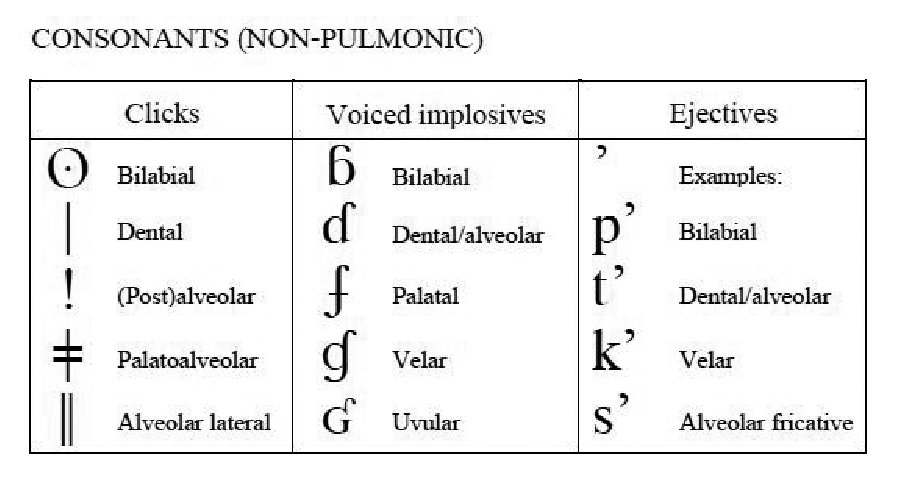
\includegraphics[scale=0.45]{material/04ipaconsonantnonpulmonic}
%		\caption{Konsonanten (Nicht Pulmonal)}
%		%\label{Zeichen1}
%	\end{figure}
	
	\begin{itemize}
		\item \textbf{VIDEO:} \href{run:material/04namaclicks.mp4}{!Nama Clicks}
	\end{itemize}
			
\end{frame}



%%%%%%%%%%%%%%%%%%%%%%%%%%%%%%%%%%%%%%%%%%%%%%%%%%%%%%%%%%%%%%%%%%%

\begin{frame}
\frametitle{IPA-Alphabet}

	\begin{figure}[H]
		\centering
		
		\includegraphics[scale=0.27]{material/04ipavowelwikicommons}
		\caption{CC BY-SA 3.0, https://en.wikipedia.org/w/index.php?curid=3368128}
		%old picture
		%\includegraphics[scale=0.45]{material/04ipavowel}
		%\caption{Vokale}
		%\label{Zeichen1}
	\end{figure}
	
\end{frame}


%%%%%%%%%%%%%%%%%%%%%%%%%%%%%%%%%%%%%%%%%%%%%%%%%%%%%%%%%%%%%%%%

\begin{frame}
\frametitle{IPA-Alphabet}

	\begin{figure}[H] %%kein lizensfreies Bild gefunden%%
		\centering
		
		\includegraphics[scale=0.5]{material/04ipatabellerepp11vokalviereck}
		\caption{Vokale für das Deutsche}
		%\label{Zeichen1}
	\end{figure}
	
\end{frame}


%%%%%%%%%%%%%%%%%%%%%%%%%%%%%%%%%%%%%%%%%%%%%%%%%%%%%%%%%%%%%%%%

\begin{frame}
\frametitle{IPA-Alphabet}

	\begin{figure}[H]
		\centering
		
		\includegraphics[scale=0.5]{material/04ipasuprasegmental}
		\caption{Suprasegmentalia}
		%\label{Zeichen1}
	\end{figure}
	
\end{frame}


%%%%%%%%%%%%%%%%%%%%%%%%%%%%%%%%%%%%%%%%%%%%%%%%%%%%%%%%%%%%%%%%
%%%%%%%%%%%%%%%%%%%%%%%%%%%%%%%%%%%%%%%%%%%%%%%%%%%%%%%%%%%%%%%%
%
\section{Artikulatorische Phonetik}
\iftoggle{toc}{
\frame{
\begin{multicols}{2}
	\tableofcontents[currentsection]
\end{multicols}
}
}
%%%%%%%%%%%%%%%%%%%%%%%%%%%%%%%%%%%%%%%%%%%%%%%%%%%%%%%%%%%%%%%%

\begin{frame}{Artikulatorische Phonetik}

	\begin{itemize}
		\item Mehrere Körperteile sind für Erzeugung von Schall nötig:
		
		\begin{itemize}
			\item[]
			\item \textbf{Initiator}: die Lunge \ras (Atmung) erzeugt Luftstrom
			\item[]
			\item \textbf{Generator}: der Kehlkopf (Larynx) mit den Stimmbändern \ras Luftstrom wird in Schwingung versetzt (Phonation)
		\end{itemize}
		
		\begin{itemize}
			\item[] Frequenz: Häufigkeit mit der die Stimmlippen schwingen bestimmt die Tonhöhe (in Hz).
			\item[]

			\ea Bei Frauen ung. 230 Hz, bei Männern 120 Hz und bei Säuglingen 400 Hz
			\z

		\end{itemize}
		
		\begin{itemize}
			\item[] \textbf{VIDEO:} \href{run:material/04TransNasalEndoscopy.mp4}{Trans-Nasal Endoscopy}
		\end{itemize}
		
	\end{itemize}
	
\end{frame}


%%%%%%%%%%%%%%%%%%%%%%%%%%%%%%%%%%%%%%%%%%%%%%%%%%%%%%%%%%%%%%%%

\begin{frame}
\frametitle{Artikulatorische Phonetik}

	\begin{itemize}
		\item \textbf{Modifikator}: Rachen-, Mund- und Nasenraum mit den verschiedenen Sprechwerkzeugen (Zunge, Lippen, weicher Gaumen) \ras unterschiedliche Stellung der Artikulationsorgane verändert den Rohschall des Kehlkopfs zu den wohlunterschiedenen Lauten (Artikulation im engeren Sinne).
	\end{itemize}
	
\end{frame}



%%%%%%%%%%%%%%%%%%%%%%%%%%%%%%%%%%%%%%%%%%%%%%%%%%%%%%%%%%%%%%%%%%%%%%%%%%%%%%%%%%%%%%%%%%%%%%%%%%%%%%%%%%%%%%%%%%%%%%%%%%%%%%%%
%
\subsection{Konsonanten}
%\frame{
%\begin{multicols}{2}
%	\tableofcontents[currentsection]
%\end{multicols}
%}
%%%%%%%%%%%%%%%%%%%%%%%%%%%%%%%%%%%%%%%%%%%%%%%%%%%%%%%%%%%%%%%%

\begin{frame}{Konsonanten}

	\begin{itemize}
		\item Konsonanten \ras Mitlaute
		\item[]
		\item Die Artikulationsorgane bilden eine \textbf{geräuschverursachende Enge} oder einen Verschluss im Ansatzrohr, d.\,h. die Luft wird oberhalb der Stimmritze (Glottis) zwischen den Stimmbändern behindert.
	\end{itemize}
	
\end{frame}


%%%%%%%%%%%%%%%%%%%%%%%%%%%%%%%%%%%%%%%%%%%%%%%%%%%%%%%%%%%%%%%%

\begin{frame}
\frametitle{Konsonanten}

\begin{minipage}{0.48\textwidth}
	\begin{figure}
	\centering
	\includegraphics[scale=0.32]{material/04phonoatonomy}
	\caption{Sagitalschnitt, By 아흔 - Own work, CC BY-SA 3.0, \url{https://commons.wikimedia.org/w/index.php?curid=2615572}}
	\end{figure}
\end{minipage}\hfill
\begin{minipage}{0.4\textwidth}
	A -- Nasenraum\\
	B -- Zahndamm \emph{Alveolen}\\
	C -- (Ober)Lippe \\
	D -- (obere) Zähne\\
	E -- Zugenspitze \emph{Apex}\\
	F -- Kehlkopf \emph{Larynx}\\
	G -- Stimmlippen \emph{Glottis}\\
	H -- harter Gaumen \emph{Palatum}\\
	I -- Zungenrücken \emph{Dorsum}\\
	J -- Gaumensegel \emph{Velum}\\
	K -- Zäpfchen \emph{Uvula}\\
	L -- Luftröhre\\ 
	M -- Speiseröhre
\end{minipage}
	
%	\begin{figure}[H] %%altes Bild%%
%		\centering
%		
%		\includegraphics[scale=0.65]{material/04sagitalschnittaltmann}
%		\caption{Sagitalschnitt \citep{Altmann&Co07a}}
%		%\label{Zeichen1}
%	\end{figure}
	
\end{frame}



%%%%%%%%%%%%%%%%%%%%%%%%%%%%%%%%%%%%%%%%%%%%%%%%%%%%%%%%%%%%%%%%
%%%%%%%%%%%%%%%%%%%%%%%%%%%%%%%%%%%%%%%%%%%%%%%%%%%%%%%%%%%%%%%%
%
\subsubsection{Konsonantenklassifikation}
%
%%%%%%%%%%%%%%%%%%%%%%%%%%%%%%%%%%%%%%%%%%%%%%%%%%%%%%%%%%%%%%%%

\begin{frame}{Konsonantenklassifikation}

	\begin{itemize}
		\item \textbf{Stimmbeteiligung} (Stimmhaftigkeit): Schwingungszustand der Stimmbänder
		
		\begin{itemize}
			\item[]
			\item \textbf{stimmhaft} \ras eng beieinander stehende Stimmbänder
			\item[]
			\item \textbf{stimmlos} \ras weit auseinander stehende Stimmbänder

			\ea \textipa{[ p ]} vs. \textipa{[ b ]}
			\z

			\item[]
			\item \textbf{Aspiration} (Behauchung): Glottis während der Verschlussphase ist weit gespreizt und schwingt mit.

			\ea \textipa{[ \super h ]}
			\z

		\end{itemize}

	\end{itemize}
	
\end{frame}



%%%%%%%%%%%%%%%%%%%%%%%%%%%%%%%%%%%%%%%%%%%%%%%%%%%%%%%%%%%%%%%%

\begin{frame}
\frametitle{Konsonantenklassifikation}

\begin{itemize}
		\item \textbf{ÜB:} Welche der folgenden Laute sind stimmhaft und welche stimmlos?

		\ea \textipa{[ d, z, f, v, g, k, P ]}
		\z
		
\end{itemize}

\end{frame}


%%%%%%%%%%%%%%%%%%%%%%%%%%%%%%%%%%%%%%%%%%%%%%%%%%%%%

\begin{frame}
\frametitle{Lösung}

\begin{itemize}
\item stimmhaft: \textipa{[ d, z, v, g ]}
\item[]
\item stimmlos: \textipa{[ f, k, P ]}
\end{itemize}
\end{frame}

%%%%%%%%%%%%%%%%%%%%%%%%%%%%%%%%%%%%%%%%%%%%%%%%%%%%%%%%%%%%%%%%

\begin{frame}
\frametitle{Konsonantenklassifikation}

	\begin{itemize}
		\item \textbf{Stellung des Gaumensegels} (des weichen Gaumens):
		
		\begin{itemize}
			\item[]
			\item Nasale Laute (\zB \textipa{ [ m , n ]}) \ras Senkung des weichen Gaumens (Velum)
			\item[]
			\item Orale Laute (\zB \textipa{ [ f , a ]}) \ras bei gehobenem Velum
		\end{itemize}
		
		\item[]
		\item \textbf{LINK:} \href{http://smu-facweb.smu.ca/~s0949176/sammy/}{Interactive Sagittal Section}
	\end{itemize}
	
\end{frame}


%%%%%%%%%%%%%%%%%%%%%%%%%%%%%%%%%%%%%%%%%%%%%%%%%%%%%%%%%%%%%%%%

\begin{frame}
\frametitle{Konsonantenklassifikation}

	\begin{itemize}
		\item \textbf{Artikulationsort} im Vokaltrakt: Ort, an dem die Luft behindert wird. Man unterscheidet darunter die nicht-beweglichen von den beweglichen Artikulatoren.

		\item[]
		\item \textbf{Nicht-bewegliche} Artikulatoren (passiver Artikulator, Artikulationsort im engeren Sinne):
			
		\begin{itemize}
			\item die oberen Zähne \ras dental
			\item[]
			\item die Alveolen (Knochendamm hinter den oberen Zähne) \ras alveolar
			\item[]
			\item der harte Gaumen (Palatum) \ras palatal
		\end{itemize}
		
	\end{itemize}
	
\end{frame}


%%%%%%%%%%%%%%%%%%%%%%%%%%%%%%%%%%%%%%%%%%%%%%%%%%%%%%%%%%%%%%%%

\begin{frame}
\frametitle{Konsonantenlassifikation}

\begin{itemize}
	\item \textbf{Bewegliche} Artikulatoren (aktiver Artikulator, Artikulationsorgan):
			
	\begin{itemize}
		\item[]
		\item weicher Gaumen (Velum) \ras velar
		\item[]
		\item das Zäpfchen (Uvula) \ras uvular
		\item[]
		\item Lippen \ras labial
		\item[]
		\item Unterkiefer
		\item[]
		\item Zunge
	\end{itemize}

\end{itemize}

\end{frame}


%%%%%%%%%%%%%%%%%%%%%%%%%%%%%%%%%%%%%%%%%%%%%%%%%%%%%%%%%%%%%%

\begin{frame}
\frametitle{Konsonantenklassifikation}

	\begin{itemize}
		\item \textbf{EXTRA-INFORMATION:}
		
		\begin{itemize}
			\item[]
			\item Bei der Artikulation mit der Zunge bildet man Untergruppen nach dem beteiligten Zungenteil:
			
			\begin{itemize}
				\item[]
				\item \textbf{koronal}: mit dem vorderen Teil der Zunge\\
				\ras \textbf{apikal}: mit der Zungenspitze\\
				\ras \textbf{laminal}: mit dem Zungenblatt (mittlerer Teil der Zunge)

				\ea \textipa{[ t, d, l, n, s, z, S, Z ]}
				\z

				\item \textbf{dorsal}: mit dem hinteren Teil der Zunge

				\ea \textipa{[ \c{c}, j, g, k, x, N, \textscr , K ]}
				\z

			\end{itemize}
						 
		\end{itemize}
		
		\item[]
		\item \textbf{LINK:} \href{http://smu-facweb.smu.ca/~s0949176/sammy/}{Interactive Sagittal Section}
	\end{itemize}
	
\end{frame}


%%%%%%%%%%%%%%%%%%%%%%%%%%%%%%%%%%%%%%%%%%%%%%%%%%%%%%%%%%%%%%%%

\begin{frame}
\frametitle{Konsonantenklassifikation}

	\begin{itemize}
		\item \textbf{Artikulationsart} (Artikulationsmodus): Art der Behinderung des Luftstroms durch die Artikulationsorgane

			\item[]
			\item \textbf{Plosive} (Verschlusslaute, Explosivlaute, stops): Totaler oraler Verschluss mit anschließender plötzlicher Lösung des Verschlusses\\
	Das Velum bleibt dabei in angehobener Position, so dass die Luft durch den Mundraum strömt.

			\ea \textipa{[ p, b, t, d, k, g, P ]}
			\z
			
			\begin{itemize}
				\item Der \textbf{Glottalverschluss} (Knacklaut) \textipa{[ P ]} entsteht durch plötzliches Öffnen der Stimmritze und kommt im Deutschen vor anlautendem Vokal eines Wortes und vor anlautendem Vokal in einer betonten Silbe vor.
			\end{itemize}
		
	\end{itemize}
	
\end{frame}


%%%%%%%%%%%%%%%%%%%%%%%%%%%%%%%%%%%%%%%%%%%%%%%%%%%%%%%%%%%%%%%%

\begin{frame}
\frametitle{Konsonantenklassifikation}

		\begin{itemize}
			\item \textbf{Frikative} (Reibelaute, Spiranten): Verengung zweier Sprechorgane, Luftstrom strömt durch die Verengung, es entsteht ein Reibegeräusch.

			\ea \textipa{[ f, v, s, z, S, Z, \c{c}, x, h, K ]}
			\z
			
			\begin{itemize}
				\item \textbf{Sibilanten} (Zischlaut): Unterklasse der Frikative mit intensivem, hochfrequentem Geräuschanteil.

				\ea \textipa{[ s, z, S ]}
				\z

		\end{itemize}
		
	\end{itemize}
	
\end{frame}


%%%%%%%%%%%%%%%%%%%%%%%%%%%%%%%%%%%%%%%%%%%%%%%%%%%%%%%%%%%%%%%%

\begin{frame}
\frametitle{Konsonantenklassifikation}

		\begin{itemize}
			\item \textbf{Affrikaten}: Plosive, die in Frikative übergehen, wobei die Verschlussphase und die Frikativphase dieselbe (oder annähernd dieselbe) Artikulationsstelle haben; d.\,h. sie sind \textbf{homorgan}.

			\ea \textipa{[ \t{pf} , \t{ts} , \t{tS} , \t{dZ} ]}
			\z

			\begin{itemize}
				\item Per Definitionem gehören der plosive und der frikative Laut einer Affrikaten \textbf{zum selben Morphem} (die kleinste Bedeutungs-tragende Einheit). Daraus ergibt sich:

				\ea \textipa{[ \t{ts} ]} in \ab{Blitz} \ras Affrikate
				\z
				
				\ea \textipa{[ \t{ts} ]} in \ab{Monats} \ras keine Affrikate
				\z

			\end{itemize}
		
		\item[]
		\item Plosive, Frikative und Affrikaten \ras \textbf{Obstruenten}
	\end{itemize}
	
\end{frame}


%%%%%%%%%%%%%%%%%%%%%%%%%%%%%%%%%%%%%%%%%%%%%%%%%%%%%%%%%%%%%%%%

\begin{frame}
\frametitle{Konsonantenklassifikation}

		\begin{itemize}
			\item \textbf{Vibranten} (trills): schnelle Folge oraler Verschlüsse
			\begin{itemize}
				\item[]
				\item Artikulationsstellen für Vibranten sehr eingeschränkt: nur bilabial, alveolar oder uvular
				\item[]
				\item Der alveolare Vibrant \textipa{[ r ]} (das sog. Zungenspitzen-R) kommt in vielen süddeutschen Varietäten vor.
				\item[]
				\item Der uvulare Vibrant \textipa{[ \textscr ]} (das gerollte Zäpfchen-R) ist eine häufige Realisierung des Deutschen \ab{r}.
			\end{itemize}
			 
	\end{itemize}
	
\end{frame}


%%%%%%%%%%%%%%%%%%%%%%%%%%%%%%%%%%%%%%%%%%%%%%%%%%%%%%%%%%%%%%%%

\begin{frame}
\frametitle{Konsonantenklassifikation}

		\begin{itemize}
			\item \textbf{Approximanten} (Öffnungslaute): Enge im Ansatzrohr (wie Frikative)\\
			Bei Approximanten gibt es nicht so eine große Nähe zwischen Artikulator und Artikulationsstelle \ras kein Reibegeräusch
			\item[]
			\item[] Zwei Unterklassen:
			
			\begin{itemize}
				\item[]
				\item \textbf{Laterale}: Verschluss in der Mundhöhlenmitte, Luft entweicht seitlich [~\textipa{l}~]
				\item[]
				\item \textbf{Gleitlaute} (zentral): zentrale Verengung aber weiter als bei Frikativen [~\textipa{w}~].\\
				(Manchmal wird [~\textipa{j}~] auch zu den Gleitlauten gezählt, da die Verengung weiter als bei anderen Frikativen ist, dies ist jedoch strittig!)
			\end{itemize}
			
		\end{itemize}	

\end{frame}


%%%%%%%%%%%%%%%%%%%%%%%%%%%%%%%%%%%%%%%%%%%%%%%%%%%%%%%%%%%%%%%%

\begin{frame}
\frametitle{Konsonantenklassifikation}

		\begin{itemize}
			\item \textbf{Nasale}: totaler oraler Verschluss (wie Plosive). Luft entweicht durch die Nase durch Senken des Velums\\
			\item[] Im Deutschen kommen 3 Nasale vor: \textipa{[ m, n, N ]}

		\item[]
		\item Vibranten, Approximanten (Laterale und Gleitlaute), Nasale und Vokale (auch die hier nicht behandelten \gqq{geschlagenen Laute} wie das span. \textipa{[ R ]}) gehören zur Gruppe der \textbf{Sonoranten}, da die Luft bei denen ungehindert ausströmen kann. Sonoranten sind \textbf{immer} stimmhaft!
		\item[]
		\item Die Klasse der l-Laute und r-Laute werden auch zu den sog. \textbf{Liquiden} zusammengefasst (im Dt. \textipa{[ l, r, \textscr ]})
	\end{itemize}
	
\end{frame}


%%%%%%%%%%%%%%%%%%%%%%%%%%%%%%%%%%%%%%%%%%%%%%%%%%%%%%%%%%%%%%%%

\begin{frame}
\frametitle{Konsonantenklassifikation}

	\begin{itemize}
		\item Für die Differenzierung der deutschen Konsonanten sind hauptsächlich 3 Merkmale wichtig:
		
		\begin{itemize}
			\item[]
			\item Stimmbeteiligung
			\item Artikulationsort
			\item Artikulationsart
		\end{itemize}
		
		\item[]
		\item \textbf{ÜB:} Beschreiben Sie die Konsonanten in den folgenden Wörtern und geben Sie die entsprechenden phonetischen Symbole an:
		\item[] Busch, malen, Maus, Achtung, Genie, zirpen, wichtig, Wald
	\end{itemize}
	
\end{frame}


%%%%%%%%%%%%%%%%%%%%%%%%%%%%%%%%%%%%%%%%%%%%%%%%%%%%%%%%%%%%%%%%
%
\subsection{Vokale}
\iftoggle{toc}{
\frame{
\begin{multicols}{2}
	\tableofcontents[currentsection]
\end{multicols}
}
}
%%%%%%%%%%%%%%%%%%%%%%%%%%%%%%%%%%%%%%%%%%%%%%%%%%%%%%%%%%%%%%%%

\begin{frame}{Vokale}

	\begin{itemize}
		\item \textbf{Vokale} (Selbstlaute) sind Laute, bei deren Artikulation die Luft ungehindert durch den Mundraum strömen kann (deswegen gehören sie zu den Sonoranten)
		\item[]
		\item Vokale sind \idR immer stimmhaft.
		\item[]
		\item Es ist umstritten, ob der sog. Schwa-Laut im Dt. \textipa{[ @ ]} stimmhaft ist, auch im Japanischen soll es stimmlose Vokale geben
	\end{itemize}
	
\end{frame}


%%%%%%%%%%%%%%%%%%%%%%%%%%%%%%%%%%%%%%%%%%%%%%%%%%%%%%%%%%%%%%%%
%%%%%%%%%%%%%%%%%%%%%%%%%%%%%%%%%%%%%%%%%%%%%%%%%%%%%%%%%%%%%%%%
%
\subsubsection{Vokalklassifikation}
%
%%%%%%%%%%%%%%%%%%%%%%%%%%%%%%%%%%%%%%%%%%%%%%%%%%%%%%%%%%%%%%%%

\begin{frame}{Vokalklassifikation}

	\begin{itemize}
		\item \textbf{Zungenhöhe} (Vokalhöhe): Grad der Zungenhebung in Richtung Gaumen

		\ea hoch: \textipa{[ i: ]}, mittel: \textipa{[ o: ]}, tief: \textipa{[ a: ]} bzw. geschlossen, halboffen, offen
		\z

		\item[]
		\item \textbf{Zungenlage} (Vokaltiefe): angehobener Teil der Zunge

		\ea vorne: \textipa{[ i: ]}, zentral: \textipa{[ a: ]}, hinten: \textipa{[ u: ]}
		\z

	\end{itemize}
	
\end{frame}


%%%%%%%%%%%%%%%%%%%%%%%%%%%%%%%%%%%%%%%%%%%%%%%%%%%%%%%%%%%%%%%%

\begin{frame}
\frametitle{Vokalklassifikation}

	\begin{itemize}
		\item \textbf{Lippenrundung}: Art der Lippenöffnung

		\ea gerundet: \textipa{[ o: ]}, ungerundet: \textipa{[ i: ]}
		\z

		\item[]
		\item\textbf{ÜB:} Lesen Sie die folgenden Wörter erst mit gerundeten danach mit gespreizten Lippen:
		\item[] Bühne, rühmen, Dünen, Stiele, Trieb, Möhre, Herd, Hefe
	\end{itemize}
	
\end{frame}


%%%%%%%%%%%%%%%%%%%%%%%%%%%%%%%%%%%%%%%%%%%%%%%%%%%%%%%%%%%%%%%%

\begin{frame}
\frametitle{Vokalklassifikation}

	\begin{itemize}
		\item \textbf{Gespanntheit} vs. Ungespanntheit der Muskeln (Länge, Vokalquantität):
		
		\begin{itemize}
			\item[]
			\item Definition 1: \textipa{[ i:, y:, u:, o: ]} \textbf{mehr Muskelspannung} als \textipa{[ I, Y, \textupsilon , O ]}\\
			(von der experimentellen Phonetik weder bestätigt noch widerlegt)
			\item[]
			\item Definition 2: mit vorverlagerter Zungenwurzel
			\item[]
			\item I.\;d.\textscr . alle tiefen Vokale \ras ungespannt (strittig!)
			\item langer tiefer Vokal \textipa{[ a: ]} \ras gespannt(?)
		\end{itemize}
		
	\end{itemize}
	
\end{frame}


%%%%%%%%%%%%%%%%%%%%%%%%%%%%%%%%%%%%%%%%%%%%%%%%%%%%%%%%%%%%%%%%

\begin{frame}
\frametitle{Vokalklassifikation}

	\begin{itemize}
	
		\item Im Deutschen: Korrelation der Gespanntheit mit der Länge.

		\ea \textipa{[ m i: t @ ]} vs. \textipa{[ m I t @ ]}
		\z

		\item In Lehnwörtern findet man auch kurze gespannte Vokale

		\ea \textipa{[ P i . d e: ]}
		\z
		
\vspace{1em}
		
		\item \textbf{Stellung des Gaumensegels}:
		
		\begin{itemize}
			\item oral
			\item nasal
			\item[]
			\item Nasalvokale kommen im Dt. nur in Lehnwörtern vor.

			\ea \textipa{[ \~a, \~o, \~E, \~\oe ]}
			\z
		
		\end{itemize}
		
	\end{itemize}
	
\end{frame}


%%%%%%%%%%%%%%%%%%%%%%%%%%%%%%%%%%%%%%%%%%%%%%%%%%%%%%%%%%%%%%%%

\begin{frame}
\frametitle{Vokalklassifikation}

	\begin{itemize}
		\item Für die Differenzierung der deutschen nativen Vokale sind hauptsächlich 4 Merkmale wichtig:
		
		\begin{itemize}
			\item[]
			\item Zungenhöhe
			\item[]
			\item Zungenlage
			\item[]
			\item Lippenrundung
			\item[]
			\item Gespanntheit (bzw. Länge)
		\end{itemize}
		
	\end{itemize}
	
\end{frame}


%%%%%%%%%%%%%%%%%%%%%%%%%%%%%%%%%%%%%%%%%%%%%%%%%%%%%%%%%%%%%%%%
%%%%%%%%%%%%%%%%%%%%%%%%%%%%%%%%%%%%%%%%%%%%%%%%%%%%%%%%%%%%%%%%
%
\subsubsection{Vokalviereck}
%\frame{
%\begin{multicols}{2}
%	\tableofcontents[currentsection]
%\end{multicols}
%}
%%%%%%%%%%%%%%%%%%%%%%%%%%%%%%%%%%%%%%%%%%%%%%%%%%%%%%%%%%%%%%%%

\begin{frame}{Vokalviereck}

	\begin{itemize}
		\item Für eine bessere Darstellung wurden die Vokale (von Daniel Jones 1920) in das sog. Vokalviereck angeordnet, welches eine stilisierte Version des Vokalraums darstellt.
	\end{itemize}

	\begin{figure}[H]
		\centering
		
		\includegraphics[scale=0.4]{material/04ipatabellerepp11vokalviereck} %%kein gutes lizensfreies Bild gefunden%%
		\caption{Vokalviereck \citep{Repp&Co12a}}
		%\label{Zeichen1}
	\end{figure}	
	
\end{frame}


%%%%%%%%%%%%%%%%%%%%%%%%%%%%%%%%%%%%%%%%%%%%%%%%%%%%%%%%%%%%%%%%
%%%%%%%%%%%%%%%%%%%%%%%%%%%%%%%%%%%%%%%%%%%%%%%%%%%%%%%%%%%%%%%%
%
\subsubsection{Monophthong, Diphthong, Triphthong}
%\frame{
%\begin{multicols}{2}
%	\tableofcontents[currentsection]
%\end{multicols}
%}
%%%%%%%%%%%%%%%%%%%%%%%%%%%%%%%%%%%%%%%%%%%%%%%%%%%%%%%%%%%%%%%%

\begin{frame}{Monophthong, Diphthong, Triphthong}

\begin{itemize}
	\item \textbf{Monophthong}

	\begin{itemize}		
		\item einzelner (langer oder kurzer) Vokal
		\item[]
	\end{itemize}
	
	\item \textbf{Diphthong} (Zwielaut, Doppellaut)
	
	\begin{itemize}		
		\item Abfolge von zwei Vokalen
		\item[]
		\item Beide Einheiten haben zusammen die gleiche Dauer wie ein einzelner langer Vokal
		\item[]
		\item Beide Vokale gehören zur selben Silbe (im Silbenkern)
		\item[]
		\item Zunge gleitet bei der Artikulation von einer Stellung in eine andere
		\item[]
		\item Laut ändert kontinuierlich seine Qualität
	\end{itemize}
	
\end{itemize}	

\end{frame}


%%%%%%%%%%%%%%%%%%%%%%%%%%%%%%%%%%%%%%%%%%%%%%%%%%%%%%%%%%%%%%%%

\begin{frame}
\frametitle{Monophthong, Diphthong, Triphthong}

	\begin{itemize}
		\item \textbf{Unterklassen} der Diphthonge:
		
		\begin{itemize}
			\item[]
			\item \textbf{fallende} (oder schließende) Diphthonge (echte deutsche Diphthonge)

			\ea \textipa{[ \t{aI} , \t{aU} , \t{OI} ]} oder \textipa{[ a\textsubarch{I} , a\textsubarch{U} , O\textsubarch{I} ]}
			\z

			\item[]
			\item \textbf{steigende} (oder öffnende) Diphthonge\\

			\ea Im Bayrischen: \textipa{[ \t{Ia} , \t{Ua} ]} oder \textipa{[ \textsubarch{I}a , \textsubarch{\textupsilon}a ]} (in \ab{liap} und \ab{guat})
			\z
			
			\ea In Fremdwörtern: \abe{Span\textit{ie}n}, \abe{Rit\textit{ua}l}, \abe{Stud\textit{iu}m}
			\z
			
			\item fallend vs. steigend \ras akustisch-auditiv
			\item schließend vs. öffnend \ras artikulatorisch
		\end{itemize}
		
	\end{itemize}
	
\end{frame}


%%%%%%%%%%%%%%%%%%%%%%%%%%%%%%%%%%%%%%%%%%%%%%%%%%%%%%%%%%%%%%%%

\begin{frame}
\frametitle{Monophthong, Diphthong, Triphthong}

\begin{itemize}
	\item[]
		
	\begin{itemize}
		\item \textbf{zentralisierende} Diphthonge (durch R-Vokalisierung \ras keine Phoneme)

		\ea \textipa{[ \t{i5} , \t{I5} , \t{e5} , \t{u5} , \t{y5} , \t{Y5} , \t{\o5} , \t{U5} , \t{o5} ]} in \abu{hier, Birke, mehr, stur, für, mürrisch, stör, knurr, Ohr}
		\z
		
	\end{itemize}

						 		
\end{itemize}
	
\end{frame}


%%%%%%%%%%%%%%%%%%%%%%%%%%%%%%%%%%%%%%%%%%%%%%%%%%%%%%%%%%%%%%%%

\begin{frame}
\frametitle{Monophthong, Diphthong, Triphthong}

\begin{itemize}
	\item \textbf{Triphthong} (Dreilaut)
	
	\begin{itemize}
		\item Abfolge von drei Vokalen im Silbenkern (?)
		\item[]
		\item Anzahl der Silben \ras unsicher
		\item[]
		\item \textbf{linear steigende}
		\item[]
		\item \textbf{linear fallende}
		\item[]
		\item mit \textbf{Umkehrpunkt}
	\end{itemize}
	
	\ea \textipa{[ \t{aI5} , \t{OI5}, \t{aU5} ]} in \ab{Eier, Steuer, Bauer}
	\z
	
\end{itemize}	

\end{frame}

	
	
%%%%%%%%%%%%%%%%%%%%%%%%%%%%%%%%%%%%%%%%%%%%%%%%%%%%%%%%%%%%%%%%
%%%%%%%%%%%%%%%%%%%%%%%%%%%%%%%%%%%%%%%%%%%%%%%%%%%%%%%%%%%%%%%%
%
\section{Übungen}
\iftoggle{toc}{
\frame{
\begin{multicols}{2}
\frametitle{~}
	\tableofcontents[currentsection]
\end{multicols}
}
}
%%%%%%%%%%%%%%%%%%%%%%%%%%%%%%%%%%%%%%%%%%%%%%%%%%%%%%%%%%%%%%%%

\begin{frame}
\frametitle{Übungen}

\begin{itemize}
	\item \textbf{ÜB:} Bilden die folgenden Vokalabfolgen Diphthonge?
		\item[] Zeit, naiv, Haus
\end{itemize}

\end{frame}


%%%%%%%%%%%%%%%%%%%%%%%%%%%%%%%%%%%%%%%%%%%%%%%%%%%%%%%%%%%%%%%%

\begin{frame}
\frametitle{Lösung}

\begin{itemize}
	\item Ja: \textipa{[ \t{ts} \t{aI} t ]} , \textipa{h \t{aU} s ]}
	\item Nein: \textipa{[ n a . P i: f ]}
\end{itemize}
\end{frame}

%%%%%%%%%%%%%%%%%%%%%%%%%%%%%%%%%%%%%%%%%%%%%%%%%%%%%
\begin{frame}
\frametitle{Übungen}

	\begin{itemize}
		
		\item \textbf{ÜB:} Transkribieren Sie die folgenden Wörter nach einer standarddeutschen Aussprache:
		
				\begin{columns}
			\column{.40\textwidth}
				\begin{enumerate}
					\item Bergsteiger
					\item Quotennote
					\item vielfaches
					\item Päckchenannahme
					\item beenden
					\item verreisen
					\item vereisen
					\item Einzahlung
					\item gehen
					\item Gästebad
				\end{enumerate} 
			\column{.40\textwidth}
				\begin{enumerate}
					\item<2> \textipa{[b\t{E5}k.St\t{aI}.g5]}
					\item<2> \textipa{[kvo:.t@n.no:.t@]}
					\item<2> \textipa{[fi:l.fa\.x@s]}
					\item<2> \textipa{[pEk.\c{c}@n.Pan.na:.m@]}
					\item<2> \textipa{[b@.PEn.d@n]}
					\item<2> \textipa{[f\t{E5}.\textscr \t{aI}.z@n]}
					\item<2> \textipa{[f\t{E5}.P\t{aI}.z@n]}
					\item<2> \textipa{[P\t{aI}n.\t{ts}a:.lUN]}
					\item<2> \textipa{[ge:.@n]}
					\item<2> \textipa{[gEs.t@.ba:t]}
				\end{enumerate} 
		\end{columns}
		
	\end{itemize}
	
\end{frame}


%%%%%%%%%%%%%%%%%%%%%%%%%%%%%%%%%%%%%%%%%%%%%%%%%%%%%%%%%%%%%%%%

\begin{frame}
\frametitle{Übungen}

	\begin{itemize}
		\item \textbf{ÜB:} Geben Sie die orthographische Transkription des folgenden Textes an:		
	\end{itemize}
	
	\begin{figure}[H]
		\includegraphics[scale=0.22]{material/04einststrittentranspompino}		
	\end{figure}
	
	\begin{itemize}
		\item \textbf{SOUND:} \href{run:material/04einststrittenaudio/04einststritten.wpl}{Text}
	\end{itemize}

	
\end{frame}


%%%%%%%%%%%%%%%%%%%%%%%%%%%%%%%%%%%%%%%%%%%%%%%%%%%%%%%%%%%%%%%%

\begin{frame}
\frametitle{Übungen}

	\begin{itemize}
		\item \textbf{ÜB:} Geben Sie die orthographische Transkription des folgenden Textes an:		
	\end{itemize}
	
	\begin{figure}[H]
		\centering
		
		\includegraphics[scale=0.22]{material/04einststrittenorthopompino}
		\caption{\citep{Pompino95a}, \citep{Kohler99a}}
		%\label{Zeichen1}
	\end{figure}	
		
\end{frame}


%%%%%%%%%%%%%%%%%%%%%%%%%%%%%%%%%%%%%%%%%%%%%%%%%%%%%%%
\begin{frame}
\frametitle{Lösung}

Einst stritten sich Nordwind und Sonne, wer von ihnen beiden wohl der Stärkere wäre, als ein
Wanderer, der in einen warmen Mantel gehüllt war, des Weges daherkam. Sie wurden einig, dass
derjenige für den Stärkeren gelten sollte, der den Wanderer zwingen würde, seinen Mantel
abzunehmen. Der Nordwind blies mit aller Macht, aber je mehr er blies, desto fester hüllte sich der
Wanderer in seinen Mantel ein. Endlich gab der Nordwind den Kampf auf. Nun erwärmte die Sonne die
Luft mit ihrem freundlichen Strahlen, und schon nach wenigen Augenblicken zog der Wanderer seinen
Mantel aus. Da musste der Nordwind zugeben, dass die Sonne von ihnen beiden der Stärkere war.

\end{frame}

%%%%%%%%%%%%%%%%%%%%%%%%%%%%%%%%%%%%%%%%%%%%%%%%%%%%%%

\begin{frame}{\textipa{[ S l U s ]}}

	\begin{itemize}
		\item \textbf{VIDEO:} \href{run:material/04vocalcordssinging.wmv}{Vocal Cords}
	\end{itemize}
	
\end{frame}


%%%%%%%%%%%%%%%%%%%%%%%%%%%%%%%%%%%%%%%%%%%%%%%%%%%%%%%%%%%%%%%%
%%%%%%%%%%%%%%%%%%%%%%%%%%%%%%%%%%%%%%%%%%%%%%%%%%%%%%%%%%%%%%%%
%
\section{Elektronische Quellen}
%\frame{
%\begin{multicols}{2}
%\frametitle{~}
%	\tableofcontents[currentsection]
%\end{multicols}
%}
%%%%%%%%%%%%%%%%%%%%%%%%%%%%%%%%%%%%%%%%%%%%%%%%%%%%%%%%%%%%%%%%

\begin{frame}{Elektronische Quellen}
	\small
	
	\begin{itemize}
		\item VIDEO -- \gqq{Spoken Pirahã with subtitles} (Zugriff: 24.10.2013): \url{http://www.youtube.com/watch?v=SHv3-U9VPAs}
		\item LINK -- \gqq{Webseite der IPA} (Zugriff: 24.10.2013): \url{http://internationalphoneticassociation.org}
		\item LINK -- \gqq{Peter Ladefoged -- A Course in Phonetics} (Alle Laute zum Testen) (Zugriff: 24.10.2013):\\ \url{http://phonetics.ucla.edu/course/chapter1/chapter1.html}
		\item VIDEO -- \gqq{!Nama Clicks} (Zugriff: 24.10.2013): \url{http://www.youtube.com/watch?v=Ophrf64fxgA&list=PL6rcWnFnBuT7BEAex2IvI6l_bjLLycxaU}
		\item VIDEO -- \gqq{Anatomical Tutorial During Trans-Nasal Endoscopy} (Zugriff: 24.10.2012): \url{http://www.youtube.com/watch?v=wjRsa77u6OU}
		\item LINK -- \gqq{Interactive Sagittal Section} (Zugriff: 27.04.2016): \url{http://smu-facweb.smu.ca/~s0949176/sammy/}
		\item VIDEO -- \gqq{Vocal Cords up close while singing} (Zugriff: 24.10.2012): \url{http://www.youtube.com/watch?v=-XGds2GAvGQ}
	\end{itemize}
	
\end{frame}


